\chapter{nEDM measurement in PSI}
\label{ch:nedm-at-psi-apparatus}

% \section{The collaboration}
The nEDM-at-PSI collaboration \note{name?} has been founded to perform an nEDM measurement in the Paul Scherrer Institute (PSI) in Villigen, Switzerland. The experiment was planned in two stages. In the first stage, the apparatus used in the ILL experiment was moved to PSI, where it was installed to benefit from a new, highly intense source of ultracold neutrons~\cite{Lauss2014}. The first stage finished in Autumn 2017, after having collected enough statistics to set the world's best limit (Fig.\,\ref{fig:nEDM_accumulated_sensitivity}). As of Spring 2018 the analysis is still ongoing.

\begin{figure}
  \centering
  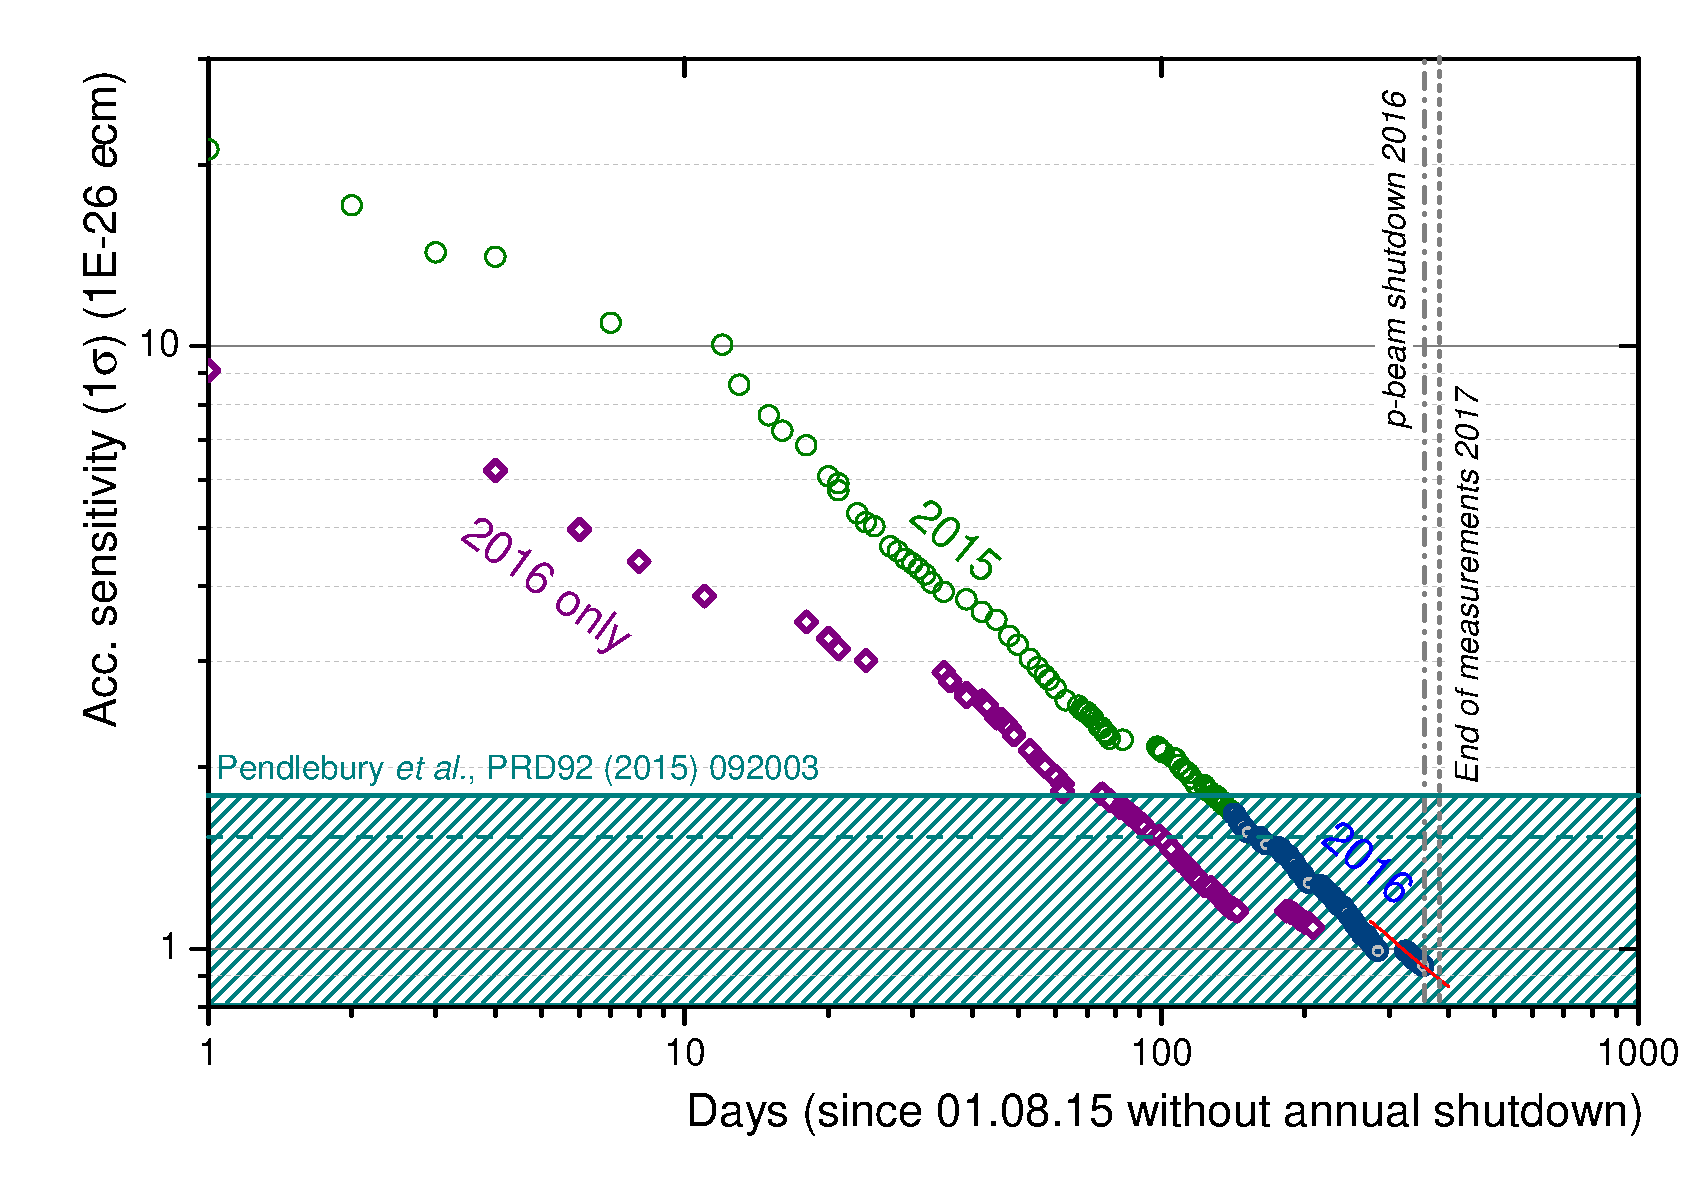
\includegraphics[width=0.8\linewidth]{gfx/nEDMatPSI/accumulated_sensitivity.pdf}
  \caption{The accumulated statistical sensitivity of the nEDM-at-PSI experiment. The sensitivity of the data collected in 2015 is shown in green, of 2015 and 2016 in blue, and only 2016 in violet. The dashed region marks the yet unexplored area below the best limit~\cite{Pendlebury2015}. Courtesy of Dr. Philipp Schmidt-Wellenburg.}
  \label{fig:nEDM_accumulated_sensitivity}
\end{figure}

Already in the first stage the apparatus underwent numerous improvements, leaving only few parts of the original. The improvements were part of the research and development plan for the second stage, a newly built apparatus called n2EDM. The new experiment, designed by the personnel experienced with running, modifying and improving the first stage, has the goal of exploring the \SI{e-27}{\elementarycharge\centi\meter} range.


\section{The apparatus}
This work focuses on the stage-one apparatus, which we now proceed do describe. A
The stage-one apparatus employed the Ramsey method with ultracold neutrons stored for the time of the precession. The neutrons produced in the source were guided with a pipe system into the storage chamber, where they underwent the Ramsey procedure. The polarisation was then measured by letting the neutrons fall into a spin-state--sensitive neutron detector. A diagram of the system is shown in Fig.\,\ref{fig:nEDM_scheme}.

\begin{figure}
  \centering
  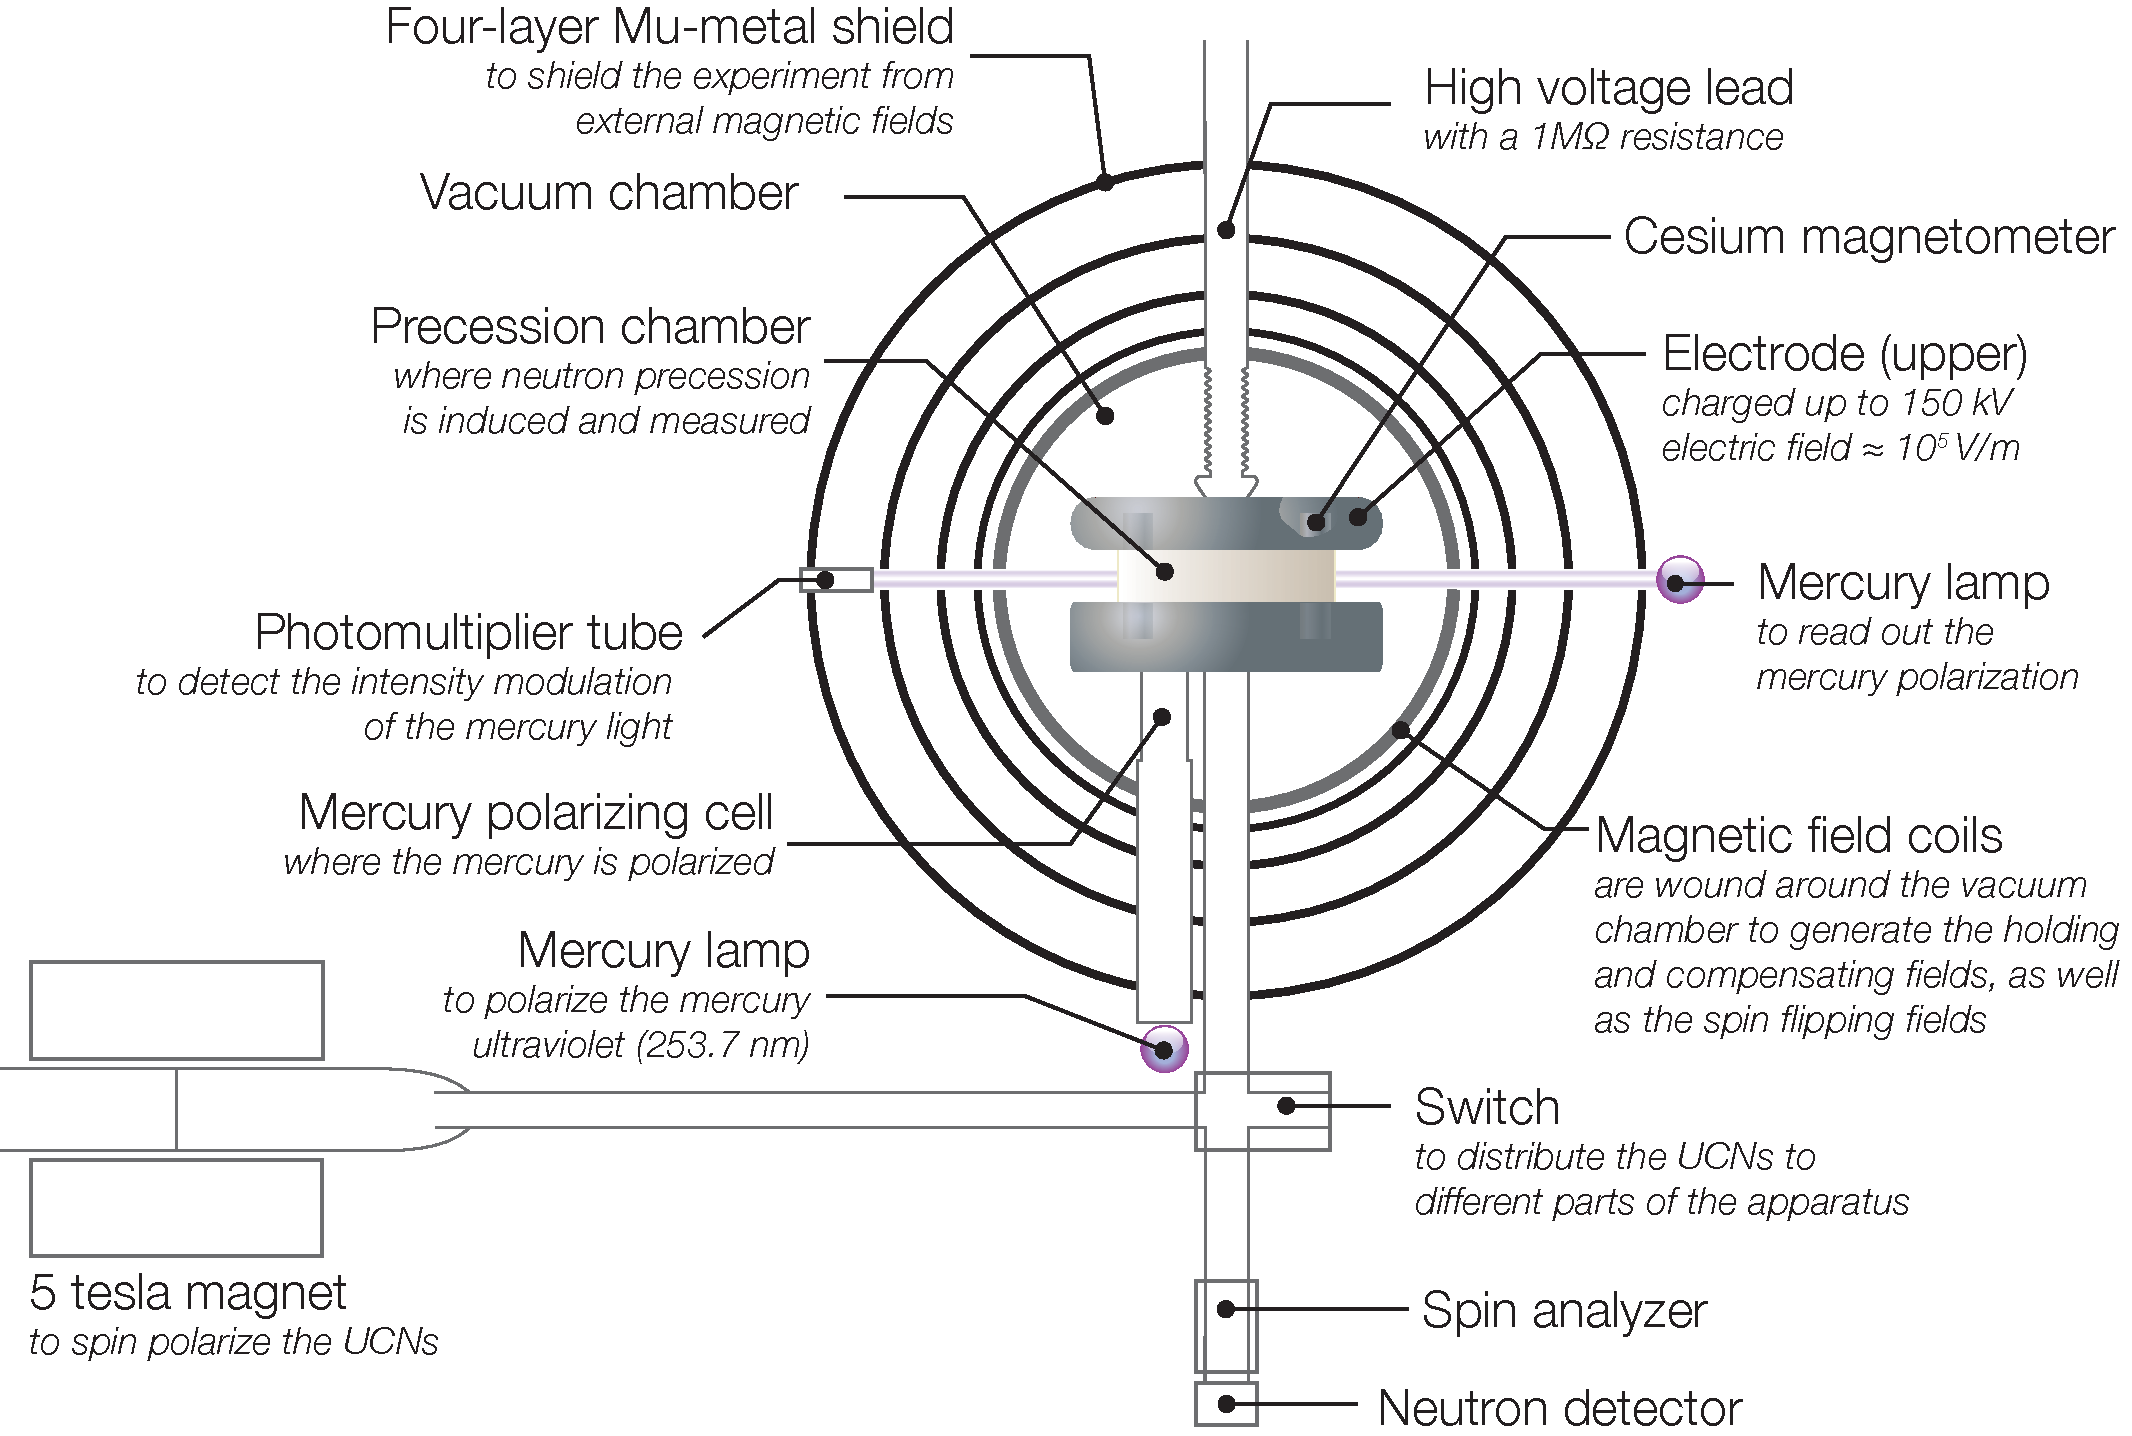
\includegraphics[width=\linewidth]{gfx/nEDMatPSI/apparatus-cartoon-main-and-sub-labels.pdf}
  \caption{The scheme of the nEDM-at-PSI apparatus. \note{Whom to credit for the image? Make my own? No\ldots}}
  \label{fig:nEDM_scheme}
\end{figure}

A single measurement cycle was triggered by a pulse of ultracold neutrons incoming from the PSI source. The neutrons were guided in metal-coated glass pipes. First they were polarised by passing a five-tesla magnet. Then a rotary three-way valve, the switch, directed the neutrons upwards into a vacuum tank, where they filled a \SI{12}{\centi\meter}-high cylindrical precession chamber. The chamber was submerged in a \SI{1}{\micro\tesla} vertical magnetic field $B_0$. The chamber was sandwiched between high-voltage electrodes, charged to \SI{132}{\kilo\volt}, which created the electric field in the chamber. Once the neutrons filled the cylinder, the entrance was shut close and the particles were stored for around \SI{200}{\second}, while undergoing the Ramsey procedure.

First, a pulse of oscillating transverse field was applied, with its amplitude and length tuned, so that the the neutrons' spins flip from the vertical orientation, along the $B_0$ field, to the horizontal plane. This set the spins into a Larmor precession.
\marginpar{The nEDM-at-PSI experiment the neutrons were dropped into two-armed detector, capable of counting both spin states simultaneously~\cite{Afach2015USSA}.}
After \SI{180}{\second} a second pulse, in phase with the first one, was applied. Then the chamber's entrance was opened, and the neutrons were allowed to fall through the switch and a spin analyser into the neutron detector.


The purpose of rest of the components, the majority, in fact, is either providing a stable magnetic field environment in the precession chamber or measuring the field.




\section{Magnetic fields}
The most important measure of stabilising the magnetic field is passive shielding. The vacuum tank, with the precession chamber in it, was covered by four layers of highly permeable material, called $\upmu$-metal.
\marginpar{The exact attenuation factor of the shield depended on the direction and varied from 1600 to 13300~\cite{Komposch2017}.}
Each layer attenuated the magnetic field changes by a factor approximately ten. High magnetic permeability of the $\upmu$-metal makes the magnetic field much rather go inside the metal and around the volume it encloses, than to penetrate into the volume. Even though $\upmu$-metal provided excellent shielding properties, it is a ferromagnetic: it distorts the field both outside and inside the shield. Also it had to be regularly demagnetised.

Inside the shield, on the vacuum chamber, there were a number of coils wound. The main magnetic field $B_0$ was produced by a cos-theta coil.
\marginpar{In an ensemble precessing in an inhomogenous field, members in different places precess at slightly different rates. This leads to depolarisation by the loss of coherence.}
Besides, there were numerous others, producing field of various shapes.
They were, on one hand, used to homogenise the field, which reduced the depolarisation rate of the neutrons,
and on the other to deliberately apply vertical gradients $\partial_z B_0$. Operating in different gradients was part of the measurement procedure and is explained later in this chapter.

The stability of the field inside the shield was in the picotesla range. The remaining variations are measured and corrected for, primarily with the mercury-based magnetometer. Below the precession chamber there was a cell containing a vapour of polarised $^{199}$Hg atoms, which was released into the precession chamber once it had been filled with neutrons.
\marginpar{In the \SI{1}{\micro\tesla} $B_0$ field the precession frequencies of neutrons and $^{199}$Hg atoms are approximately \SI{30}{\hertz} and \SI{8}{\hertz}, respectively. The respective spin-flip pulses affect the other spices only very slightly.}
There, a dedicated spin-flip pulse of an oscillating transverse magnetic field started their coherent precession, which was read on-line optically~\cite{FertlThesis,Komposch2017}. A mercury discharge lamp shone a circularly polarised light through the precession chamber onto a photomultiplier tube. As the mercury atoms' photon-capture cross-section depended on the phase of the precession, the transparency of the chamber to the polarised light oscillated at the mercury's Larmor frequency. The oscillating signal of the photomultiplier was then analysed to estimate its frequency, proportional to the $B_0$ field, as averaged by the mercury atoms.

The mercury comagnetometer may seem a an ideal measure to correct the neutron measurement for the drifts of the magnetic field, as the two spices filled exactly the same volume. Only, not exactly. The ultracold neutrons were slow enough to be affected by the gravity, which shifted their centre of mass around \SI{2.4}{\milli\meter} relative to the homogeneous mercury vapour~\note{Afach2014magmoment}. In a presence of a vertical gradient, the two spices saw different fields. Additional, smaller systematic effects related to this magnetometer, are discussed in~\cite{Afach2014magmoment}.

A way to measure vertical gradients, as well as other high-order components of the magnetic field, was provided by an array of Caesium magnetometers. These sensors were located inside the electrodes---seven in the top one, nine in the bottom one. Each magnetometer was a cell filled with Caesium vapour, through which a circuraly polarised light, delivered with a light guide, shone at \SI{45}{\degree} inclination angle. The light simultaneously polarised the atoms and, as it met a surface of a photodiode behind the cell, probed their precession. A coil wound around the cell, axial with the light beam, was driven in a feedback loop with the diode's signal to resonantly drive the Larmor precession. Even though the magnetometers measured only the magnitude of the magnetic field, they provided information about the higher-order components of the field thanks to their distribution around the chamber. For example, one could na\"\i vely estimate the vertical gradient $\partial_z B_z$ by evaluating the average readings of the sensors in each electrode, taking the difference and dividing by the vertical separation. Actually, the high-order field terms, including the vertical gradient, were obtained by fitting a second-order parametrization of the magnetic field to the readings of the sensors~\cite{WurstenThesis}.

Now we proceed to explain how all these components came together to perform a measurement of the electric dipole moment of the neutron.



\section{Measurement procedure}
\begin{figure}
  \centering
  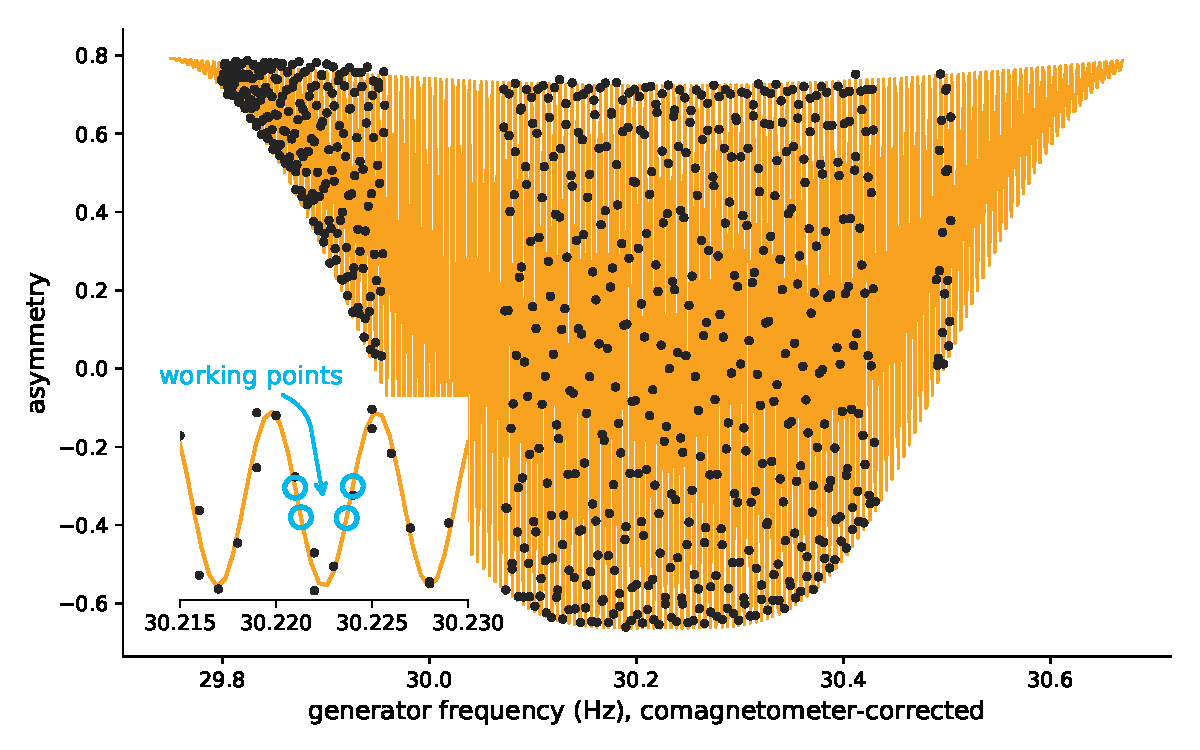
\includegraphics[width=0.8\linewidth]{gfx/nEDMatPSI/ramsey_scan.pdf}
  \caption{A scan of the Ramsey resonance curve in the nEDM-at-PSI experiment---the asymmetry is measured as the function of the detuning of the spin-flip generator's frequency. Black points depict the measured points, orange line is the fit of the theoretical model. In the inset the central fringe is enlarged and the working points are marked, which is where the experiment took data during normal operation. The generator frequency has been corrected with the $^{199}$Hg comagnetometer using the formula $\nu_\text{generator} / \nu_\text{Hg} \times \overline{\nu_\text{Hg}}$, where $\overline{\nu_\text{Hg}}$ is the average over the scan.}
  \label{fig:ramsey_scan}
\end{figure}

Recall the Ramsey method (Fig.\,\ref{fig:nEDM_Ramsey_principle}). Two coherent pulses of a transverse oscillating field are applied to an ensemble of polarised neutrons, with a period of free precession in between. Measuring the polarisation after the second pulse as the function of the frequency of the transverse field yields a resonance curve. The curve measured in the nEDM-at-PSI experiment is reproduced in Fig.\,\ref{fig:ramsey_scan}. Comparing it with Ramsey's original curve (Fig.\,\ref{fig:nEDM_Ramsey_original_curve}) summarises fifty years of progress in measuring the electric dipole moment of the neutron.

In the normal operation not the whole curve was sampled, but only the region most sensitive to the position of the central fringe---its steepest slope. In Fig.\,\ref{fig:nEDM_Ramsey_principle} the four \emph{working points} are marked, which the experiment was programmed to aim at. Assuming all the data are taken in this most sensitive region the sensitivity for the nEDM is~\note{FertlThesis}:
\begin{equation}
  \sigma(d_\text{n}) = \frac{\hbar}{ 2 \alpha E T \sqrt{N} } \ ,
\end{equation}
where $\alpha$ is the relative height of the curve ($\alpha = 1$ means the curve spanning from $-1$ to $1$ in asymmetry), $E$ is the strength of the electric field, $T$ is the duration of the free precession (\SI{180}{\second}, its inverse is the width of the fringes), and $N$ is the counting statistics. It is the statistical limit on the sensitivity---the value obtained from the analysis will be slightly worse.

Each cycle of the experiment, filling in the neutrons, performing the Ramsey procedure and counting them, sampled one of the working points on the resonance curve. Assuming that the only parameter that changed between the cycles was the position of the resonance (due to drifts of the field), one could estimate the position of the central fringe, the neutron precession frequency $\nu_\text{n}$ for each cycle. In other words, the neutrons were a very accurate magnetometer operating on a cycle basis.
% The resonance frequency $f_n^{\,0}$ is determined with a fit of the resonance curve. Because the points are probed one after another, it is only possible after a set of data points, \emph{cycles}, have been measured. In order to extract the neutron precession frequency for each individual \emph{cycle}, one assumes that the only parameter of the resonance curve that varies on a cycle--to--cycle basis is the position of the resonance. With this assumption the shape of the curve, fitted to the whole set of \emph{cycles}, is used to calculate back the resonant frequency in each \emph{cycle} of the set.

Naturally, measuring the magnetic field with the neutrons was not the goal. It was the, much, much smaller, if any, effect of the electric field on the precession frequency that the experiment was after. To even out the variations in $\nu_\text{n}$, its ratio to the frequency of the comagnetometer's mercury atoms $\nu_\text{Hg}$ was used instead:
\marginpar{This correction was already included in the depiction of the resonance curve in Fig.\,\ref{fig:ramsey_scan}.}
\begin{equation}
  \label{eq:Rdefinition}
  R \equiv \frac{\nu_\text{n}}{\nu_\text{Hg}} = \frac{\mu_\text{n}}{\mu_\text{Hg}} \pm \left( d_\text{n} - \frac{\mu_\text{n}}{\mu_\text{Hg}} \, d_\text{Hg} \right) \frac{2 E}{ h  \nu_\text{Hg}} + \Delta \ ,
\end{equation}
where the signs correspond to the parallel and anti-parallel configuration of the magnetic and electric fields.
It is immediately visible that $R$ is sensitive to $d_\text{n}$ just as $\nu_\text{n}$, but the fluctuations due the changes of the magnetic field are suppressed. \note{Put the derivation as an appendix? Maybe}
\marginpar{$R$ is actually sensitive to $d_\text{n} - \frac{\mu_\text{n}}{\mu_\text{Hg}} \, d_\text{Hg}$, but it has been measured that $|d_\text{Hg}| < \SI{7.4e-30}{\elementarycharge\centi\meter}$~\cite{PhysRevLett.116.161601}.}
$\Delta$ encapsulates all higher-order terms and systematic effects. In particular, the already mentioned effect due to the gravitational sag of the neutrons' population, relative to the geometrical centre of the chamber, in combination with a vertical gradient of the magnetic field.
% Together with the UCNs there is a polarised $^{199}$Hg gas precessing. Its precession is monitored with light, allowing for direct determination of the $^{199}$Hg Larmor frequecy and thus the magnetic field strength. In order to cancel the first-order magnetic field changes one looks at the value:
% \begin{equation}
%   R := f_n / f_{Hg} \ .
% \end{equation}
% However, the UCNs are cold enough to have their centre of mass shifted downwards a few centimeters by the gravity. The $^{199}$Hg gas, being much hotter then the UCNs, fills the precession volume homogeneously. In a presence of a vertical magnetic field gradient this causes the two species to see different magnetic fields.

% The largest effect in $\Delta$ has to do with the gradient of the magnetic field. The neutrons and mercury did not sample exactly the same field. The mercury vapour was at room temperature and filled the precession volume homogeneously. At the same time, the ultracold neutrons had an energy of only around \SI{300}{\nano\electronvolt}, while their gravitational potential is $m_\text{n} = \SI{102}{\nano\electronvolt\per\meter}$ steep~\cite{Zenner2013}. In effect, they filled, and sampled, the bottom of the chamber more then the top. The difference between centres of masses of the mercury and the neutrons was around \SI{4}{\mili\meter}

\begin{figure}
  \centering
  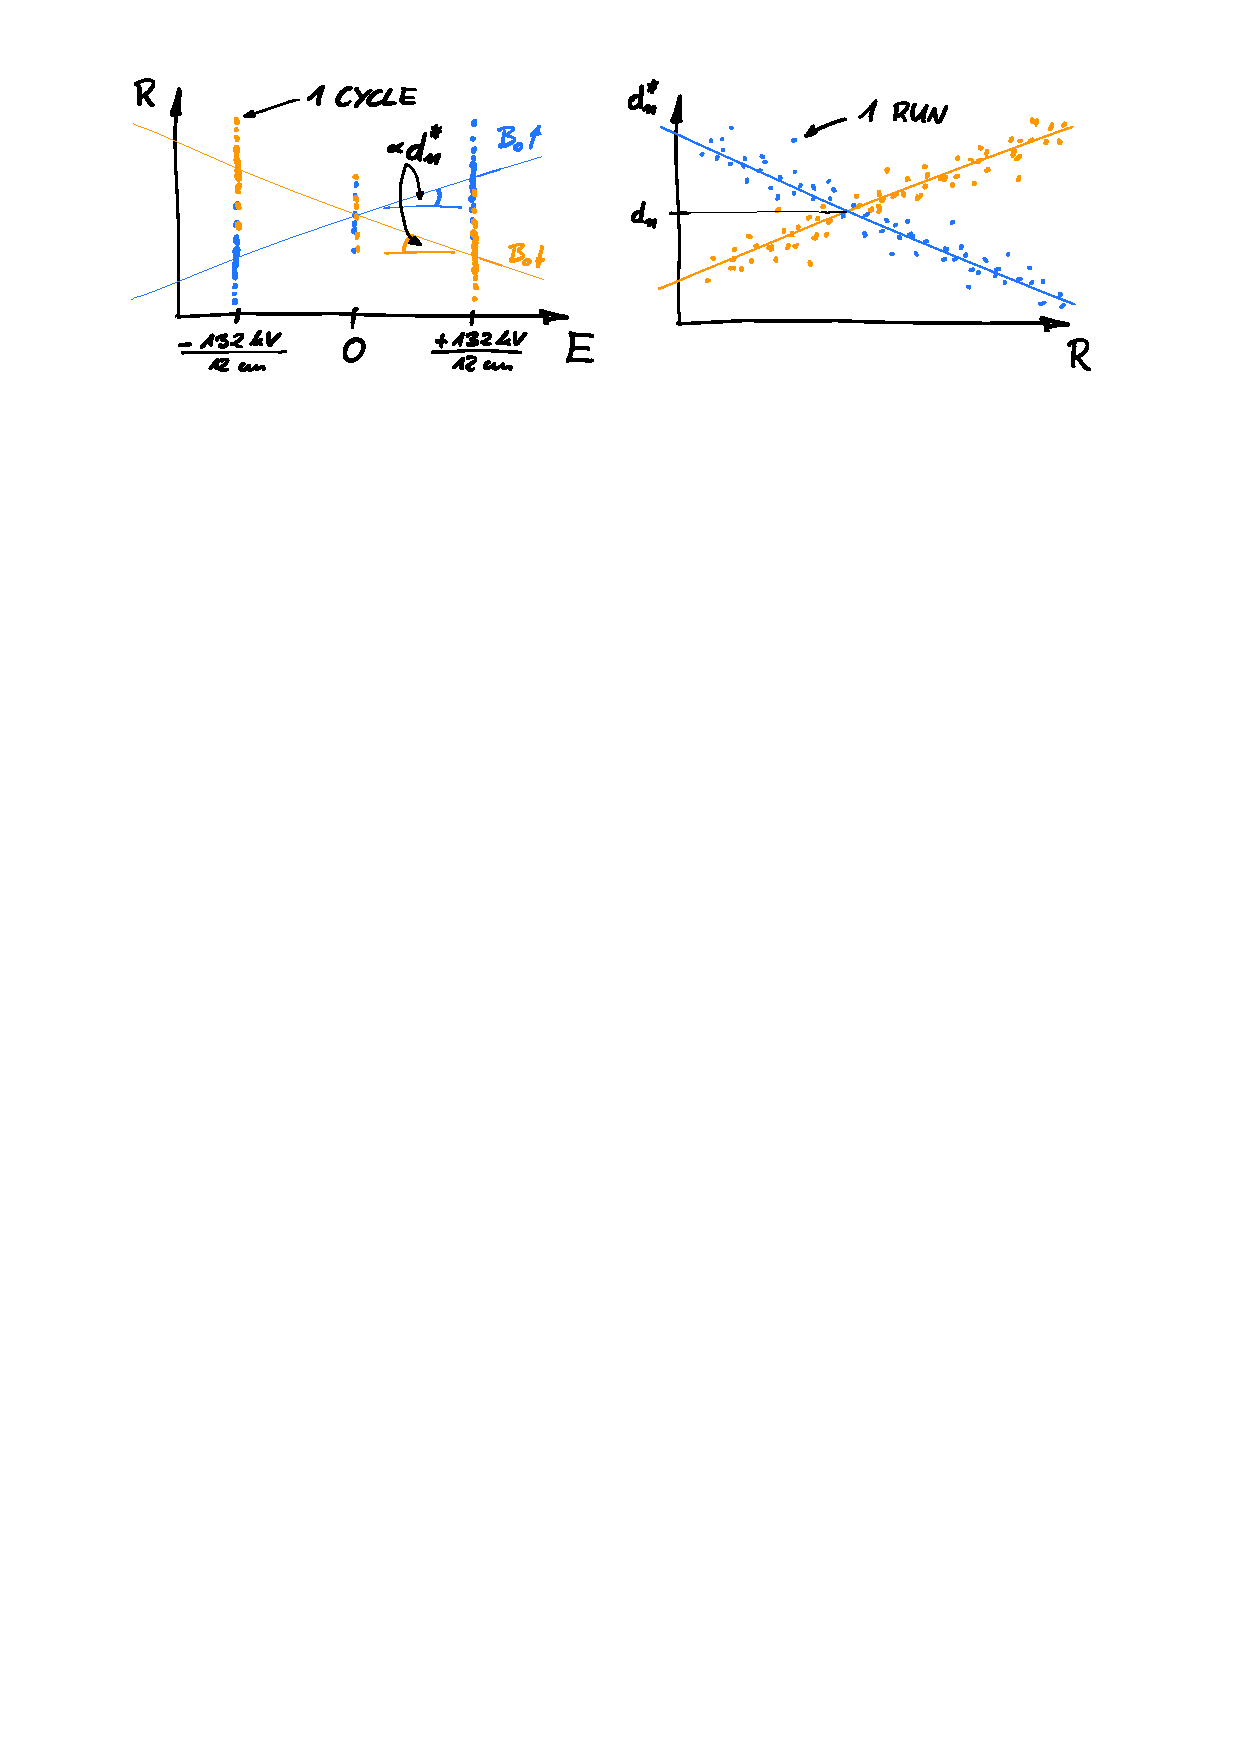
\includegraphics[width=0.8\linewidth]{gfx/nEDMatPSI/crossing_lines.pdf}
  \caption{\ldots}
  \label{fig:crossing_lines}
\end{figure}

To get the $d_n$ estimate the electric field needed to be modulated. The experiment automatically reversed the polarisation of the electric field every 72 cycles. In between the two polarisations a few cycles were measured without the electric field (a total of 10\% of the data, which are not sensitive to the nEDM). Then a linear model of  $R$ vs. $E$ yielded an estimate of $d_n$ (Eq.\,\ref{eq:Rdefinition}).

Those estimates, however, still contained a large contribution of a systematic effect. As a result of a conspiracy between radial magnetic field components and rotating magnetic components arising from the Lorentz transformation of the large electric field into the rest frame of the mercury atoms, a frequency shift proportional to the applied electric field was observed, mimicking the effect of a non-zero electric dipole moment of the neutron, a false EDM. This effect is, however, directly proportional to the gradient of the applied vertical magnetic field $\partial_z B_z$, and reverses with the sign of the applied magnetic field. The false EDM effect has been analysed in more detail in \cite{Pendlebury2004,PhysRevA.71.032104,PhysRevA.73.014101} and a direct measurement of this effect was made in~\cite{Afach2015falseEDM}.

The solution was to operate in different gradients and then interpolate to the effect-free zero gradient. Every few hundred cycles a different gradient (up to \SI{60}{\pico\tesla\per\centi\meter}) was set.
%We set the magnetic configuration (homogenise the field, maybe mention the variometer method), apply a gradient (one of i don't remember how many), calibrate the Cs magnetometers (marginnote why) and measure continuously cycle after cycle in this configuration.
% We call a set of data taken in one configuration of the magnetic field a \emph{sequence}.
Finally, a for each direction of the magnetic field, a linear regression $d_n$ vs $R$, $R$ itself being an estimate of the gradient, was performed. The vertical position of the intersection of the two lines corresponded to the $d_n$ measured at zero gradient, free from this systematic effect.

% In the nEDM experiment at PSI data taking is divided into \emph{runs}. A single \emph{run} is carried out automatically with, in most cases, no human intervention. The machine cycles through the working points by itself. Also the charging of the electrodes creating the electric field is automatised. In between \emph{runs} manual interference happens, most importantly the magnetic field vertical gradient is altered.

In order to mitigate the bias due to the human factor, the nEDM experiment implements \emph{data blinding}. The data is artificially altered in a way that mimics a non--zero neutron electric dipole moment, big enough to be visible in the data. The exact value is secret and will be revealed only after the analysis is complete.

\note{A nice wrap-up paragraph here.}











% Description of the experimental setup and the measurement procedure.

% \subsection{The Sussex-RAL-ILL Room Temperature Neutron Electric Dipole Moment Experiment}
% \note{NA: this subsection is still a very early draft, I know there are still formatting issues and blanks}

% \note{This first bit is paraphrased from C.A. Baker et al., Apparatus for Measurement of the Electric Dipole Moment of the Neutron using a Cohabiting Atomic-Mercury Magnetometer}

% \note{MR: This should probably be made much shorter.}

% Most experiments to measure the static electric dipole moment of the neutron use magnetic resonance techniques to observe the Larmor precession of free neutrons in parallel and antiparallel magnetic and electric fields. The Hamiltonian of an uncharged spin $1/2$ particle in an electric and a magnetic field is:
% \begin{equation}
% H = - 2\vec{S} \cdot (\mu \vec{B} + d \vec{E})
% \end{equation}
% In the case of parallel and antiparallel magnetic and electric fields, this gives a precession frequency of:
% \begin{equation}
% h\nu = -2\mu B \mp 2dE
% \end{equation}
% In the presence of a non-zero EDM, when the direction of the applied electric field is reversed relative to the magnetic field we expect a shift in the precession frequency of
% \begin{equation}
% \delta \nu _0 = −\frac{4d_n E_0}{h} .
% \end{equation}
% In the Sussex-RAL-ILL Room Temperature experiment, polarised ultracold neutrons produced at the fundamental physics beamline at the ILL high flux reactor were stored in a material bottle (a cylinder of diameter 235mm and height 120mm), wherein their precession frequency in parallel and antiparallel combinations of electric and magnetic fields was measured using the Ramsey Technique. To combat drifts in the magnitude of the applied magnetic field, a cohabiting magnetometer of atomic $^{199}$Hg was used, and analysis was done by considering the ratio of neutron and mercury precession frequencies, “$R$”.

% Each measurement sequence (“cycle”) consisted of a filling period, a first $\pi/2$ pulse to rotate the neutron spins into the horizontal plane, a 130s period of free precession, a second $\pi/2$ pulse to project the spins onto the z axis, and an emptying period where the number of spin-up and spin-down neutrons were counted. The precession of the mercury during the free precession period was measured by observing the modulation of the absorption of light from a mercury discharge lamp \note{is it actually a discharge lamp?}. Each cycle lasted in total x minutes. Many cycles were taken at each fixed magnetic field configuration over the course of between 1 and 73 hours (a “run”), while the direction of the applied electric field was reversed every 20 cycles. From each run a value of the neutron to mercury frequency ratio $R$ was extracted, as well as a value of the apparent EDM.

% As a result of a conspiracy between radial magnetic field components and rotating magnetic components arising from the Lorentz transformation of the large applied electric field into the rest frame of the mercury atoms, a frequency shift proportional to the applied electric field was observed, mimicking the effect of a non-zero electric dipole moment of the neutron --- a “false EDM”. This effect is, however, directly proportional to the gradient of the applied vertical magnetic field dBz/dz, and reverses with the sign of the applied magnetic field. The false EDM effect has been analysed in more detail in \note{cite false edm paper(s)} and a direct measurement of this effect was made in \note{cite false edm measurement}.

% As the ILL experiment had no direct measurement of the vertical gradient, the measurement of the neutron to mercury frequency ratio was instead used as a proxy. Due to the extremely low energy of the ultracold neutron population, the centre of mass of the neutron population sags a little below the centre of the precession chamber. The relatively hot population of mercury atoms does not suffer from this effect, so there is an effective height difference $\Delta h \approx 3.7 \mathrm{mm}$ between the neutron and mercury populations. Thus, the ratio of neutron to mercury frequencies depends (to first order) on the vertical gradient like: \note{MR: We might want to get rid of the stacked fraction for clarity.}
% \begin{equation}
%   R = R_0 \left( 1 + \Delta h  \frac{\frac{\mathrm{d}B_z}{\mathrm{d}z}}{B_{0}} \right).
%   \label{eq:R}
% \end{equation}
% This frequency shift does not uniformly affect the entire neutron population: the effect is much greater for the lowest energy neutrons which have a lower centre of mass. This causes a departure from the linear relation above; however, in the low vertical gradient regime ($\lesssim 30 \mathrm{pT/cm}$) in which most of the data was taken, the effect is almost exactly linear. This effect is described more thoroughly in [cite grav depol papers].

% To correct for these false EDMs in static EDM searches, the “crossing lines” procedure was adopted.  For each direction of the magnetic field, the measured EDM value was plotted against the measured neutron to mercury frequency ratio. Barring other systematic shifts, it is considered that the vertical gradient is zero where these lines cross. Other effects arising from transverse magnetic fields, the rotation of the earth and cause additional frequency shifts in the neutrons or in the cohabiting magnetometer, which can \note{PH: no it isn't -- there are still systematics from e.g. transverse fields, which can move the crossing point away from dB/dz=0, in addition to effects such as Earth's rotation that result in a vertical shift of the crossing point...]}, and therefore a measurement of the neutron electric dipole moment independent of the false EDM effect and of the neutron to mercury frequency ratio independent of the gravitational shift can be extracted. In the rest of the run-level analysis, we work with data where these false EDM effects have been subtracted. Further systematic effects shift the measured neutron to mercury frequency ratio or the measured EDM value, however these effects can be assumed to have been constant throughout the entire experimental measurement period, and so will not be further explored in this analysis. Systematic effects affecting the static analysis of the ILL experiment are explored in depth in [cite reanalysis] and [cite apparatus paper].

% \note{MR: Need to mention explicitly, that the average $d_n$ over a run is measured (though not exactly, it is only over the free precession periods), and this is how it is treated in the Monte Carlo simulations.}


% \section{nEDM @ PSI data taking scheme}
% The nEDM experiment at PSI probes the Ramsey resonance curve of ultra--cold neutrons (\emph{UCNs}). Its operation consists of subsequent \emph{cycles}, wherein an ensemble of polarised \emph{UCNs} undergoes a Ramsey cycle in a magnetic field. At the end the polarisation of the ensemble is measured. The measurement is performed in a controllable electric field, which takes up three values: parallel to the magnetic field, antiparallel to it and zero. The electric field configuration is altered every couple of tens of cycles.

% The Ramsey resonance curve of the neutrons is probed only in four \emph{working points}, as shown in Fig.\,\ref{fig:axions_working_points}. The points lie on the curve's steep slope. Thereby the resonance position is determined more precisely then it would should the curve be probed homogeneously or close to the resonance.

% \begin{figure}[bth]
%   \myfloatalign
%   \subfloat
%   [The \emph{working points} method. The plot depicts the measured neutron polarisation in function of the $pi/2$ pulses frequency. The frequencies are normalised by appropriate gyromagnetic ratios.]
%   {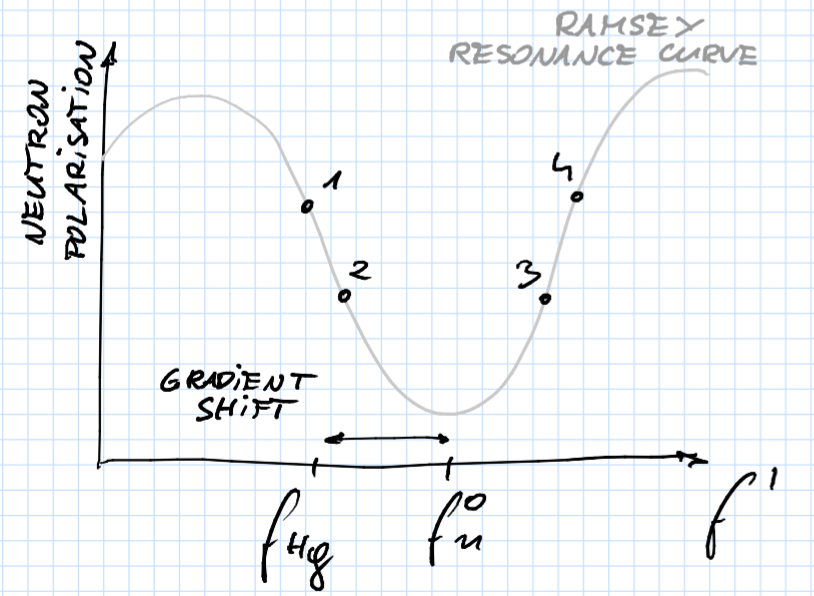
\includegraphics[width=.45\linewidth]{gfx/axions/data_taking_working_points}}
%   \quad
%   \subfloat
%   [The \emph{working points} are probed subsequently.]
%   {\label{fig:example-b}
%   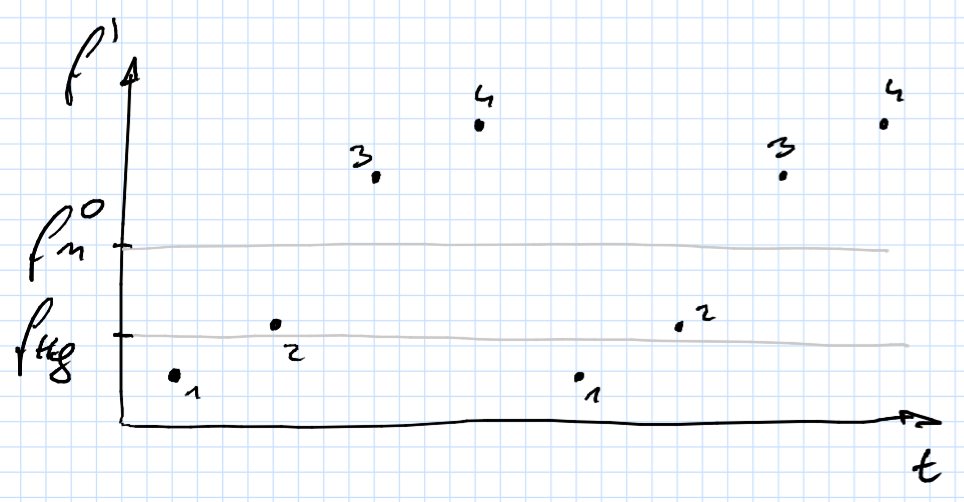
\includegraphics[width=.45\linewidth]{gfx/axions/data_taking_working_points_time}}
%   \caption{The principle of working points}
%   \label{fig:axions_working_points}
% \end{figure}

% The resonance frequency $f_n^{\,0}$ is determined with a fit of the resonance curve. Because the points are probed one after another, it is only possible after a set of data points, \emph{cycles}, have been measured. In order to extract the neutron precession frequency for each individual \emph{cycle}, one assumes that the only parameter of the resonance curve that varies on a cycle--to--cycle basis is the position of the resonance. With this assumption the shape of the curve, fitted to the whole set of \emph{cycles}, is used to calculate back the resonant frequency in each \emph{cycle} of the set.

% Together with the UCNs there is a polarised $^{199}$Hg gas precessing. Its precession is monitored with light, allowing for direct determination of the $^{199}$Hg Larmor frequecy and thus the magnetic field strength. In order to cancel the first-order magnetic field changes one looks at the value:
% \begin{equation}
%   R := f_n / f_{Hg} \ .
% \end{equation}
% However, the UCNs are cold enough to have their centre of mass shifted downwards a few centimeters by the gravity. The $^{199}$Hg gas, being much hotter then the UCNs, fills the precession volume homogeneously. In a presence of a vertical magnetic field gradient this causes the two species to see different magnetic fields.

% In the nEDM experiment at PSI data taking is divided into \emph{runs}. A single \emph{run} is carried out automatically with, in most cases, no human intervention. The machine cycles through the working points by itself. Also the charging of the electrodes creating the electric field is automatised. In between \emph{runs} manual interference happens, most importantly the magnetic field vertical gradient is altered.

% In order to mitigate the bias due to the human factor, the nEDM experiment implements \emph{data blinding}. The data is artificially altered in a way that mimics a non--zero neutron electric dipole moment, big enough to be visible in the data. The exact value is secret and will be revealed only after the analysis is complete.
